% Template for ICASSP-2021 paper; to be used with:
%          spconf.sty  - ICASSP/ICIP LaTeX style file, and
%          IEEEbib.bst - IEEE bibliography style file.
% --------------------------------------------------------------------------
\documentclass[entropy,article,submit,pdftex,moreauthors]{Definitions/mdpi} 

\usepackage{amssymb,amsmath,amsfonts,amsthm}
\usepackage{graphicx}
\usepackage{stmaryrd}
\usepackage[utf8]{inputenc}
\usepackage[T1]{fontenc}
\usepackage{tikz-cd}
\usepackage{mathtools}
\usepackage{algorithm}
\usepackage{algpseudocode}
\usepackage{diagbox}
\usepackage{tikzscale}
\usepackage[framemethod=TikZ]{mdframed}

\newcommand{\R}{\ensuremath{\mathbb{R}}}
\newcommand{\C}{\ensuremath{\mathbb{C}}}
\newcommand{\K}{\ensuremath{\mathbb{K}}}
\newcommand{\Q}{\ensuremath{\mathbb{Q}}}
\newcommand{\N}{\ensuremath{\mathbb{N}}}
\newcommand{\Z}{\ensuremath{\mathbb{Z}}}
\newcommand{\usph}[1]{\ensuremath{\mathbb{S}^{#1}}}
\newcommand{\Aff}{\ensuremath{\text{Aff}}}
\newcommand{\aff}{\ensuremath{\mathfrak{aff}}}
\newcommand{\gl}{\ensuremath{\mathfrak{gl}}}
\newcommand{\GL}{\ensuremath{\text{GL}}}
\newcommand{\homfunc}[2]{\ensuremath{\text{Hom}\left(#1,#2\right)}}
\newcommand{\comp}[2]{\ensuremath{\text{H}\left(#1,#2\right)}}
\newcommand{\homology}[3]{\ensuremath{\text{H}^{#1}\left(#2,#3\right)}}
\newcommand{\frakg}{\ensuremath{\mathfrak{g}}}
\newcommand{\pairc}[2]{\ensuremath{\left\langle #1,#2 \right\rangle_+}}
\newcommand{\paircs}[2]{\ensuremath{\left\langle #1,#2 \right\rangle_-}}
\newcommand{\pairct}[2]{\ensuremath{\left\langle #1,#2 \right\rangle_\theta}}
\newcommand{\cbracket}[2]{\ensuremath{\left\llbracket #1,#2 \right\rrbracket_c}}
\newcommand{\dbracket}[2]{\ensuremath{\left\llbracket #1,#2 \right\rrbracket_d}}
\newcommand{\lieder}[2]{\ensuremath{\mathcal{L}_#1 #2}}
\newcommand{\parder}[2]{\ensuremath{\frac{\partial #1}{\partial #2}}}
\newcommand{\gmet}[2]{\ensuremath{g\left(#1, #2  \right)}}
\newcommand{\pullg}[2]{\ensuremath{\tilde{g}\left(#1, #2  \right)}}
\newcommand{\nnet}[2]{\ensuremath{\mathcal{N}\left( #1,#2 \right)}}
\newcommand{\mnet}[1]{\ensuremath{\mathcal{N}_{W}\left( #1\right)}}
\newcommand{\lc}{\ensuremath{\nabla^{\text{lc}}}}
\newcommand{\fnet}{\ensuremath{\mathcal{N}_W}}
\newcommand{\kldiv}[2]{\ensuremath{\textit{KL}\left( #1,#2 \right)}}
\newcommand{\im}{\ensuremath{\textsf{im }}}
\DeclareMathOperator{\ad}{ad}
\DeclareMathOperator{\trace}{\ensuremath{\text{Tr}}}
\DeclareMathOperator{\ext}{\ensuremath{\text{Ext}}}

% Definitions.
% --------------------
% Math symbol font matha
\DeclareFontFamily{U}{matha}{\hyphenchar\font45}
\DeclareFontShape{U}{matha}{m}{n}{
      <5> <6> <7> <8> <9> <10> gen * matha
      <10.95> matha10 <12> <14.4> <17.28> <20.74> <24.88> matha12
      }{}
\DeclareSymbolFont{matha}{U}{matha}{m}{n}
\DeclareFontSubstitution{U}{matha}{m}{n}

% Math symbol font mathb
\DeclareFontFamily{U}{mathx}{\hyphenchar\font45}
\DeclareFontShape{U}{mathx}{m}{n}{
      <5> <6> <7> <8> <9> <10>
      <10.95> <12> <14.4> <17.28> <20.74> <24.88>
      mathx10
      }{}
\DeclareSymbolFont{mathx}{U}{mathx}{m}{n}
\DeclareFontSubstitution{U}{mathx}{m}{n}

% Symbol definition
\DeclareMathDelimiter{\vvvert}{0}{matha}{"7E}{mathx}{"17}


\setcounter{MaxMatrixCols}{20}

\theoremstyle{plain}
\newtheorem{corollary}[theorem]{Corollary}
\newtheorem{lemma}[theorem]{Lemma}
\newtheorem{proposition}[theorem]{Proposition}

\theoremstyle{definition}
\newtheorem{definition}[theorem]{Definition}
\newtheorem{example}[theorem]{Example}
\newtheorem{remark}[theorem]{Remark}
\newtheorem{fact}[theorem]{Fact}

\newcommand{\E}{\mathbb{E}}
\newcommand{\p}{\mathbb{P}}

\newcommand{\A}{\mathcal{A}}
\newcommand{\B}{\mathcal{B}}
\newcommand{\Cc}{\mathcal{C}}
\newcommand{\D}{\mathcal{D}}
\newcommand{\F}{\mathcal{F}}
\newcommand{\Ic}{\mathcal{I}}
\newcommand{\Lc}{\mathcal{L}}
\newcommand{\M}{\mathcal{M}}
\newcommand{\Oc}{\mathcal{O}}
\newcommand{\Pc}{\mathcal{P}}
\newcommand{\Sc}{\mathcal{S}}
\newcommand{\X}{\mathcal{X}}
\newcommand{\Y}{\mathcal{Y}}

\newcommand{\Bij}{\mathfrak{S}}
\newcommand{\Df}{\mathfrak{D}}
\newcommand{\Ff}{\mathfrak{F}}
\newcommand{\I}{\mathfrak{I}}
\newcommand{\Kf}{\mathfrak{K}}

\newcommand{\KL}{\textnormal{KL}}
\newcommand{\Ot}{\textnormal{O}}
\newcommand{\rank}{\textnormal{rank\:}}
\newcommand{\rg}{\textnormal{rg}}
\newcommand{\rk}{\textnormal{rk}}
\newcommand{\Sh}{\textnormal{SH}}
\newcommand{\sign}{\textnormal{sign}}
\newcommand{\Sl}{\textnormal{SL}}
\newcommand{\Sp}{\textnormal{sp}}
\newcommand{\Span}{\textnormal{span}}
\newcommand{\Spo}{\textnormal{SO}}
\newcommand{\Sym}{\textnormal{Sym}}
\newcommand{\vol}{\textnormal{vol}}

\newcommand{\gb}{\overline{g}}
\newcommand{\Gb}{\overline{G}}
\newcommand{\nablab}{\overline{\nabla}}
\newcommand{\nablat}{\widetilde{\nabla}}
\newcommand{\II}{\mathrm{I\!I}}

%=================================================================
% MDPI internal commands - do not modify
\firstpage{1} 
\makeatletter 
\setcounter{page}{\@firstpage} 
\makeatother
\pubvolume{1}
\issuenum{1}
\articlenumber{0}
\pubyear{2023}
\copyrightyear{2023}
%\externaleditor{Academic Editor: Firstname Lastname}
\datereceived{ } 
\daterevised{ } % Comment out if no revised date
\dateaccepted{ } 
\datepublished{ } 
%\datecorrected{} % For corrected papers: "Corrected: XXX" date in the original paper.
%\dateretracted{} % For corrected papers: "Retracted: XXX" date in the original paper.
\hreflink{https://doi.org/} % If needed use \linebreak
%\doinum{}
%\pdfoutput=1 % Uncommented for upload to arXiv.org
% Authors, for the paper (add full first names)
%\Author{Firstname Lastname $^{1,\dagger,\ddagger}$\orcidA{}, Firstname Lastname $^{2,\ddagger}$ and Firstname Lastname $^{2,}$*}
\Author{Loïc Shi-Garrier$^{1,\ddagger}$ , Nidhal Carla Bouaynaya$^{2}$, Daniel Delahaye${3}$ }
\address{$^{\star}$ Ecole Nationale de l'Aviation Civile, Université de Toulouse, France \\
$^{\dagger}$ Dept. of Electrical and Computer Engineering, Rowan University, New Jersey, USA }
%\longauthorlist{yes}

% MDPI internal command: Authors, for metadata in PDF
\AuthorNames{Loïc Shi-Garrier, Nidhal Carla Bouaynaya, Daniel Delahaye}

% MDPI internal command: Authors, for citation in the left column
\AuthorCitation{Shi-Garrier, L., Bouaynaya, N., Delahaye, D.}
% If this is a Chicago style journal: Lastname, Firstname, Firstname Lastname, and Firstname Lastname.

% Affiliations / Addresses (Add [1] after \address if there is only one affiliation.)
%\address{%
%$^{1}$ \quad Affiliation 1; e-mail@e-mail.com\\
%$^{2}$ \quad Affiliation 2; e-mail@e-mail.com}

\address{%
$^{1}$ \quad ENAC, Université de Toulouse, 7, Avenue Edouard Belin, Toulouse, France; loic.shi-garrier@enac.fr\\
$^{2}$ \quad Dept. of Electrical and Computer Engineering, Rowan University, New Jersey, USA ; bouaynaya@rowan.edu\\
$^{3}$ \quad ENAC, Université de Toulouse, 7, Avenue Edouard Belin, Toulouse, France; loic.shi-garrier@enac.fr}
% Contact information of the corresponding author
\corres{Correspondence: loic.shi-garrier@enac.fr}

% Title.
% ------
\Title{ADVERSARIAL ROBUSTNESS WITH PARTIAL ISOMETRY}
%
% Single address.
% ---------------
%\name{Author(s) Name(s)\thanks{Thanks to XYZ agency for funding.}}

%
% For example:
% ------------
%\address{School\\
%	Department\\
%	Address}
%
% Two addresses (uncomment and modify for two-address case).
% ----------------------------------------------------------
%\twoauthors
%  {A. Author-one, B. Author-two\sthanks{Thanks to XYZ agency for funding.}}
%	{School A-B\\
%	Department A-B\\
%	Address A-B}
%  {C. Author-three, D. Author-four\sthanks{The fourth author performed the work
%	while at ...}}
%	{School C-D\\
%	Department C-D\\
%	Address C-D}
%
\abstract{
Despite their outstanding performance, deep learning models still lack robustness guarantees, notably in the face of adversarial examples. This major weakness hinders their trustworthiness and prevents the introduction of these learning systems in critical domains where a certain level of robustness must be certified. In this paper, we present an information geometric framework to derive a precise robustness criteria for $l_2$ white-box attacks in a multi-class classification setting. We endow the output space with the Fisher information metric and derive a criteria on the input-output Jacobian to ensure robustness. We show that model robustness can be achieved by constraining the model to be partially isometric around the training points. The approach is tested on MNIST and CIFAR-10 against adversarial attacks. It is shown to be significantly more robust than defensive distillation and Jacobian regularization for medium-sized perturbations and more robust than adversarial training for large perturbations, while still maintaining desired accuracy.
}
\keyword{
Adversarial robustness, Information geometry, Fisher information metric, Multi-class classification.
}
\begin{document}
%\ninept
%
\maketitle
%
%
%
\section{Introduction}
\label{sec:intro}

% The machine learning community has started to study the robustness problems of machine learning models, neural networks in particular.
One of the motivations for studying machine learning robustness
 is the high sensitivity of neural networks to adversarial attacks, i.e., small perturbations 
 in the input data that are able to fool a network. Adversarial attacks have been shown to be both 
 ubiquitous and transferable \citep{szegedyIntriguingPropertiesNeural2014},
  \citep{goodfellowExplainingHarnessingAdversarial2015}, \citep{DBLP:conf/iclr/MadryMSTV18}. 
  Beyond the security threat, adversarial attacks are the evidence of the dramatic lack of robustness
   in machine learning models \citep{carliniEvaluatingRobustnessNeural2017}, \citep{Gilmer2018}.
    Without robustness, trustworthiness in machine learning is impossible \citep{liTrustworthyAIPrinciples2023}.

%This method consists in constraining the information ball to contain the Euclidean ball such that a perturbation bounded in $l_2$ norm is also bounded in information distance, and this bound is controlled. This condition is enforced by bounding the spectral norm of the Jacobian matrix with respect to the input.
%As a proof-of-concept, we first focus on $l_2$ white-box attacks against multi-class classification tasks; but the approach could be extended to more general settings, e.g., unrestricted attacks and black-box attacks, as well as to other supervised learning tasks.

In this paper, we shed an information geometric perspective to adversarial robustness in machine learning models. We show that robustness can be achieved by encouraging the model to be isometric in the orthogonal space of the kernel of the pullback Fisher metric. We subsequently formulate a regularization defense method for adversarial robustness. We focus on $l_2$ white-box attacks against multi-class classification tasks; but the approach could be extended to more general settings, e.g., unrestricted attacks and black-box attacks, as well as to other supervised learning tasks. The regularized model is evaluated on MNIST and CIFAR-10 against PGD $l_\infty$ attacks and AutoAttack \citep{croceReliableEvaluationAdversarial2020} with $l_\infty$ and $l_2$ norms. Comparisons with unregularized model, defensive distillation \citep{papernotDistillationDefenseAdversarial2016}, Jacobian regularization \citep{hoffmanRobustLearningJacobian2019}, and Fisher information regularization \citep{shenDefendingAdversarialAttacks2019} show significant improvement in robustness. Moreover, the regularized model is able to ensure robustness for larger perturbations compared to adversarial training.
% We pay special attention to the computational efficiency of the method since we hope that it could be used in real-world applications.

The remaining of this paper is organized as follows. Section \ref{sec:def} introduces the notations and definitions. Then, a sufficient condition for adversarial robustness at a sample point is derived. Section \ref{sec:cond} presents our method to approximate the robustness condition. The method relies on encouraging the model to be isometric in the orthogonal complement of the kernel of the pullback of the FIM. Section \ref{sec:exp} presents several experiments to evaluate the proposed method. Section \ref{sec:dis} discusses the results in the lights of related work on adversarial defense. Finally, section \ref{seq:conclu} concludes the paper and suggests potential extensions of this work. Section \ref{sec:proof} provides the proofs of the results stated in the earlier sections.

%---------------------------------------------------------------------------------------------------------------

\section{Notations and definitions}
\label{sec:def}

\subsection{Notations}

Let $d, c \in \N^*$ such that $d \geq c > 1$. Let $m = c-1$. In the learning framework, $d$ will be the dimension of the input space, while $c$ will be the number of classes. \\
% Let $\M_{m,d}(\R)$ be the set of real matrices of dimension $m \times d$. \\
% Let $\Sc^+_m(\R)$ be the set of symmetric positive-definite real matrices of dimension $m \times m$. \\
% Let $\Sc_d(\R)$ be the set of symmetric positive-semidefinite real matrices of dimension $d \times d$. \\
% Let $\GL_m(\R)$ be the set of non-singular real matrices of dimension $m \times m$. \\
% Let $\Oc_m(\R)$ be the set of real orthogonal matrices of dimension $m \times m$. \\
The range of a matrix $M$ is denoted $\rg(M)$, its rank is denoted $\rk(M)$. \\
% and its spectrum is denoted $\Sp(M)$. \\
The Euclidean norm (i.e., $l_2$ norm) is denoted $\| \cdot \|$. \\
We use the notation $\delta_{ij} = 1$ if $i=j$ and 0 otherwise. \\
% If $M_1$ and $M_2$ are two symmetric matrices, then $M_1 \preceq M_2$ means that $M_2 - M_1$ is positive semidefinite. \\
% If $M$ is any matrix, its spectral norm (i.e., largest singular value) is denoted $\|M\|_2$. Moreover, we write $\|M\|_1 = \max_{1 \leq j \leq n} \sum_{i=1}^m |M_{ij}|$ and $\|M\|_\infty = \max_{1 \leq i \leq m} \sum_{j=1}^n |M_{ij}|$. We write $(M)_+$ the maximum between 0 and the largest eigenvalue of $M$. If $r$ is any real number, we write $(r)_+ = \max\{0, r\}$. \\
% For any real-valued function $h_1$, its gradient at a point $x$ is denoted $\partial_x h_1$. \\
% For any vector-valued function $h_2$, its Jacobian matrix at a point $x$ is denoted $\nabla_x h_2$. \\
We denote the components of a vector $v$ by $v^i \in \R$ with a superscript. Smooth means $C^{\infty}$.

\subsection{Definitions}

Consider a multi-class classification task. Let $\X \subseteq \R^d$ be the \emph{input domain}, and let $\Y  = \{1, \dots, c\} \subset \N$ be the set of labels for the classification task. For example, in MNIST, we have $\X = [0,1]^d$ (with $d=784$) and $c=10$. We assume that $\X$ is an $d$-dimensional embedded smooth connected submanifold of $\R^d$.
\begin{definition}[Probability simplex]
    \label{def:simplex}
    Define the \emph{probability simplex} of dimension $m$ by:
    \small
    \begin{equation*}
        \Delta^m = \left\{\theta \in \R^c : \forall k \in \{1, \dots, c\}, \theta^k > 0 \text{ and } \sum_{i=1}^c \theta^i = 1 \right\}.
    \end{equation*}
    \normalsize
    $\Delta^m$ is a smooth submanifold of $\R^c$ of dimension $m=c-1$. When we write $\theta \in \Delta^m$, we see $\theta$ as having $m$ coordinates: $\theta = (\theta^1, \dots, \theta^m)$. Then, we define $\theta^c = 1 - \sum_{i=1}^m \theta^i$.
\end{definition}
A machine learning model (e.g., a neural network) is often seen as assigning a label $y \in \Y$ to a given input $x \in \X$. Instead, in this work, we see a model as assigning the \emph{parameters} of a random variable $Y$ to a given input $x \in \X$. The random variable $Y$ has a probability density function $p_\theta$ belonging to the \emph{family of $c$-dimensional categorical distributions} $\Sc = \{p_\theta : \theta \in \Delta^m\}$.

$\Sc$ can be endowed with a differentiable structure by using $p_\theta \in \Sc \mapsto (\theta^1, \dots, \theta^m) \in \R^m$ as a global coordinate system. Hence, $\Sc$ becomes a smooth manifold of dimension $m$ (more details on this construction can be found in \citep{amariDifferentialGeometricalMethodsStatistics1985}, Chapter 2). We can identify $p_\theta$ with $(\theta^1, \dots, \theta^m)$.

We see any machine learning model as a smooth map $f: \X \rightarrow \Delta^m$ that assigns to an input $x \in \X$, the parameters $\theta=f(x) \in \Delta^m$ of a $c$-dimensional categorical distribution $p_\theta \in \Sc$. In practice, a neural network produces a vector of logits $s(x)$. Then, these logits are transformed into the parameters $\theta$ with the softmax function: $\theta = \textnormal{softmax}(s(x))$.

In order to study the sensitivity of the predicted $f(x) \in \Delta^m$ with respect to the input $x \in \X$, we need to be able to measure distances both in $\X$ and in $\Delta^m$. In order to measure distances on smooth manifolds, we need to equip each manifold with a Riemannian metric.

First, we consider $\Delta^m$. As described above, we see $\Delta^m$ as the family of categorical distributions. A natural Riemannian metric for $\Delta^m$ (i.e., a metric that reflects the statistical properties of $\Delta^m$) is the \emph{Fisher information metric} (FIM).
\begin{definition}[Fisher information metric]
    \label{def:fim}
    For each $\theta \in \Delta^m$, the \emph{Fisher information metric} (FIM) $g$ defines a \emph{symmetric positive-definite bilinear form} $g_\theta$ over the tangent space $T_\theta\Delta^m$. In the \emph{standard coordinates} of $\R^c$, we have, for all $\theta \in \Delta^m$ and for all \emph{tangent vectors} $v,w \in T_\theta \Delta^m$:
    \begin{equation*}
    %    g_\theta(v, w) = \sum_{i,j=1}^{c-1} \left(\frac{\delta_{ij}}{\theta^i} + \frac{1}{\theta^c} \right) d\theta^i(v) \otimes d\theta^j(w)
        g_\theta(v, w) = v^T G_\theta w,
    \end{equation*}
    where $G_\theta$ is the \emph{Fisher information matrix} for parameter $\theta \in \Delta^m$ defined by:
    \begin{equation}
        G_{\theta, ij} = \frac{\delta_{ij}}{\theta^i} + \frac{1}{\theta^c}.
    \end{equation}
    For any $\theta \in \Delta^m$, the matrix $G_\theta$ is \emph{symmetric positive-definite and non-singular} (Proposition 1.6.2 in \citep{calinGeometricModelingProbability2014}). The FIM induces a distance on $\Delta^m$ called the \emph{Fisher-Rao distance} denoted $d(\theta_1, \theta_2)$ for any $\theta_1, \theta_2 \in \Delta^m$.
\end{definition}
The FIM has two remarkable property. First, it is the ``infinitesimal distance" of the the \emph{relative entropy} (Theorem 4.4.5 in \citep{calinGeometricModelingProbability2014}), which is the loss function used to train a multi-class classification model. The other remarkable property of the FIM is Chentsov's theorem \citep{cencovAlgebraicFoundationMathematical1978} claiming that the FIM is the \emph{unique} Riemannian metric on $\Delta^m$ that is invariant under sufficient statistics (up to a multiplicative constant).

Now, we consider $\X$. Since we are studying adversarial robustness, we need a metric that formalizes the idea that two close data points must be ``indistinguishable" from a human perspective (or any other relevant perspective). A natural choice is the \emph{Euclidean metric} induced from $\R^d$ on $\X$.
\begin{definition}[Euclidean metric]
    We consider the \emph{Euclidean space} $\R^d$ endowed with the \emph{Euclidean metric} $\gb$. It is defined in the standard coordinates of $\R^d$ for all $x \in \R^d$ and for all tangent vectors $v,w \in T_x \R^d$ by:
    \begin{equation*}
        \gb_x(v,w) = v^T w,
    \end{equation*}
    thus its matrix is the identity matrix of dimension $d$ denoted $I_d$. The Euclidean metric induces a distance on $\R^d$ that we will denote with the $l_2$-norm: $\|x_1 - x_2 \|$ for any $x_1, x_2 \in \R^d$.
\end{definition}
\noindent \textbf{From now on, we fix}:
\begin{itemize}
    \item a smooth map $f : (\X, \gb) \rightarrow (\Delta^m, g)$. We denote by $f^i$ the $i$-th component of $f$ in the standard coordinates of $\R^c$.
    \item a point $x \in \X$.
    \item a positive real number $\epsilon > 0$.
\end{itemize}

\begin{definition}[Euclidean ball]
    Define the Euclidean open ball centered at $x$ with radius $\epsilon$ by:
    \begin{equation*}
        \overline{b}(x, \epsilon) = \left\{ z \in \R^d : \|z-x\| < \epsilon \right\}.
    \end{equation*}
\end{definition}

\begin{definition}
    Define the set (Figure \ref{fig:opti}):
    \begin{equation*}
        \A = \left\{ \theta \in \Delta^m : \arg \max_i \theta^i = \arg \max_i f^i(x)\right\}.
    \end{equation*}
    For simplicity, assume that $f(x)$ is not on the ``boundary" of $\A$, such that $\arg \max_i f^i(x)$ is well defined.
\end{definition}

\begin{definition}[Geodesic ball of the FIM]
    Let $\delta > 0$ be the Fisher-Rao distance between $f(x)$ and $\Delta^m \setminus \A$ (Figure \ref{fig:sufficient}). \\
    Define the geodesic ball centered at $f(x) \in \Delta^m$ with radius $\delta$ by:
    \begin{equation*}
        b(f(x), \delta) = \left\{ \theta \in \Delta^m : d(f(x), \theta) \leq \delta \right\}.
    \end{equation*}
    In section \ref{seq:delta}, we propose a efficient approximation of $\delta$.
\end{definition}

\begin{definition}[Pullback metric]
    On $\X$, define the \emph{pullback metric} $\tilde{g}$ of $g$ by $f$. In the standard coordinates of $\R^d$, $\tilde{g}$ is defined for all tangent vectors $v,w \in T_x\X$ by:
    \begin{equation*}
        \tilde{g}_x(v,w) = v^T J_x^T G_{f(x)} J_x w,
    \end{equation*}
    where $J_x$ is the Jacobian matrix of $f$ at $x$ (in the standard coordinates of $\R^d$ and $\R^c$). Define the matrix of $\tilde{g}_x$ in the standard coordinates of $\R^d$ by:
    \begin{equation}
        \widetilde{G}_x = J_x^T G_{f(x)} J_x.
    \end{equation}
\end{definition}

\begin{definition}[Geodesic ball of the pullback metric]
    Let $\tilde{d}$ be the distance induced by the pullback metric $\tilde{g}$ on $\R^d$. We can define the geodesic ball centered at $x$ with radius $\delta$ by:
    \begin{equation*}
        \tilde{b}(x, \delta) = \left\{ z \in \R^d : \tilde{d}(x, z) \leq \delta \right\}.
    \end{equation*}
\end{definition}

\subsection{Robustness condition}
\label{sec:res}

\begin{figure}%[!htb]
    \begin{minipage}{0.42\textwidth}
        \centering
        \includegraphics[width=\textwidth]{figures/opti.tikz}
        \caption{$\epsilon$-robustness at $x$ is enforced if and only if $f(\overline{b}(x, \epsilon)) \subseteq \A$.}
        \label{fig:opti}
    \end{minipage}\hfill
    \begin{minipage}{0.42\textwidth}
        \centering
        \includegraphics[width=\textwidth]{figures/sufficient.tikz}
        \caption{$\epsilon$-robustness at $x$ is enforced if $\overline{b}(x, \epsilon) \subseteq \tilde{b}(x, \delta)$.}
        \label{fig:sufficient}
    \end{minipage}
    \vspace{-1em}
\end{figure}

\begin{definition}[Robustness]
We say that $f$ is $\epsilon$-robust at $x$ if:
\begin{equation}
\label{eq:robust_condition}
    \forall z \in \R^d, \|z - x\| < \epsilon \Rightarrow f(z) \in \A. 
\end{equation}
Equivalently, we can write (Figure \ref{fig:opti}):
\begin{equation}
    f(\overline{b}(x, \epsilon)) \subseteq \A.
\end{equation}
\end{definition}

\begin{proposition}[Sufficient condition for robustness]
    \label{prop:sufficient}
    If $\overline{b}(x, \epsilon) \subseteq \tilde{b}(x, \delta)$, then $f$ is $\epsilon$-robust at $x$ (Figure \ref{fig:sufficient}).
\end{proposition}
Our goal is to start from Proposition \ref{prop:sufficient} and make several assumptions in order to derive a condition that can be efficiently implemented.

Working with geodesic balls $\overline{b}(x, \epsilon)$ and $\tilde{b}(x, \delta)$ is intractable, so our first assumption consists in using an ``infinitesimal" condition by restating Proposition \ref{prop:sufficient} in the tangent space $T_x \X$ instead of working directly on $\X$.

\begin{definition}
    In $T_x\X$, define the Euclidean ball of radius $\epsilon$ by:
    \begin{equation*}
        \overline{\B}_x(0, \epsilon) = \left\{v \in T_x\X : \gb_x(v,v) = v^T v \leq \epsilon^2 \right\}.
    \end{equation*}
\end{definition}

\begin{definition}
    In $T_x\X$, define the $\tilde{g}_x$-ball of radius $\delta$ by:
    \begin{equation*}
        \widetilde{\B}_x(0, \delta) = \left\{v \in T_x\X : \tilde{g}_x(v,v) = v^T \widetilde{G}_x v \leq \delta^2 \right\}.
    \end{equation*}
\end{definition}

\noindent \textbf{Assumption 1.} We replace Proposition \ref{prop:sufficient} by:
\begin{equation}
\label{eq:as1}
    \overline{\B}_x(0, \epsilon) \subseteq \widetilde{\B}_x(0, \delta).
\end{equation}
For small enough $\delta$, Eq. (\ref{eq:as1}) implies $\epsilon$-robustness at $x$. However, contrary to Proposition \ref{prop:sufficient}, Eq. (\ref{eq:as1}) does not offer any guarantee on the $\epsilon$-robustness at $x$ for arbitrary $\delta$.
\begin{proposition}
\label{prop:as1}
    Eq. (\ref{eq:as1}) is equivalent to:
    \begin{equation}
        \label{eq:as1-2}
        \forall v \in T_x\X, \quad \tilde{g}_x(v,v) \leq \frac{\delta^2}{\epsilon^2} \gb_x(v,v).
    \end{equation}
\end{proposition}
Since $m < d$, the Jacobian matrix $J_x$ has rank smaller or equal to $m$. Thus, since $G_{f(x)}$ has full rank, $\widetilde{G}_x = J_x^T G_{f(x)} J_x$ has rank at most $m$ (when $J_x$ has rank $m$).

\noindent \textbf{Assumption 2.} The Jacobian matrix $J_x$ has full rank equal to $m$.

\section{Derivation of the regularization method}
\label{sec:cond}

\subsection{The partial isometry condition}

\noindent \textbf{In order to simplify the notations,} we replace:
\begin{itemize}
    \item $J_x$ by $J$ which is a full-rank $m \times d$ real matrix.
    \item $G_{f(x)}$ by $G$ which is a $m \times m$ symmetric positive definite real matrix.
    \item $\widetilde{G}_x$ by $\widetilde{G}$ which is a $d \times d$ symmetric positive semidefinite real matrix.
\end{itemize}
We define $D = (\ker(\widetilde{G}))^\perp$. We will use the two following facts.
\begin{fact}
\label{fact1}
    \begin{equation*}
        D = \rg(J^T) = \left(\ker(J)\right)^\perp = \left(\ker(J^T G J)\right)^\perp
    \end{equation*}
\end{fact}

\begin{fact}
    \label{fact2}
    $J^T G J$ is symmetric positive semidefinite. Thus, by the spectral theorem, the eigenvectors associated to its nonzero eigenvalues are all in $D = \rg(J^T)$. \\
    In particular, since $\rk(J)=m$, there exists an orthonormal basis of $T_x\X$, denoted $\B = (e_1, \dots, e_m, e_{m+1}, \dots, e_d)$, such that each $e_i$ is an eigenvector of $J^T G J$ and such that $(e_1, \dots, e_m)$ is a basis of $D = \rg(J^T)$ and $(e_{m+1}, \dots, e_d)$ is a basis of $\ker(J)$.
\end{fact}
The set $D = \rg(J^T)$ is a $m$-dimensional subspace of $T_x\X$. $\tilde{g}_x$ does not define an inner product\footnote{In particular, the set $\widetilde{\B}_x(0, \delta)$ is not bounded, i.e., it is a cylinder rather than a ball.} on $T_x\X$ because $\widetilde{G}$ has a nontrivial kernel of dimension $d-m$. However, when restricted to $D$, $\tilde{g}_x|_D$ defines an inner product.
\begin{definition}
    We define the restriction of $\widetilde{\B}_x(0, \delta)$ to $D$:
    \begin{equation*}
        \widetilde{\B}_D(0, \delta) = \left\{v \in D : v^T \widetilde{G} v \leq \delta \right\}
    \end{equation*}
\end{definition}

\begin{definition}
    We define the restriction of $\overline{\B}_x(0, \epsilon)$ to $D$:
    \begin{equation*}
        \overline{\B}_D(0, \epsilon) = \left\{v \in D : v^T v \leq \epsilon^2 \right\}.
    \end{equation*}
\end{definition}

\noindent \textbf{Assumption 3.} We replace Eq. (\ref{eq:as1}) with:
\begin{equation}
    \label{eq:as2}
    \overline{\B}_{D}(0, \epsilon) = \widetilde{\B}_{D}(0, \delta).
\end{equation}
Eq. (\ref{eq:as2}) is the limit case of Eq. (\ref{eq:as1}), in the sense that if Eq. (\ref{eq:as2}) holds, then $\widetilde{\B}_x(0, \delta)$ is the smallest possible $\tilde{g}_x$-ball (for the inclusion) such that Eq. (\ref{eq:as1}) holds.
\begin{proposition}
    \label{prop:as2}
    Eq. (\ref{eq:as2}) is equivalent to:
    \begin{equation}
        \label{eq:as2-2}
        \forall v \in D, \quad \tilde{g}_x(v,v) = \frac{\delta^2}{\epsilon^2} \gb_x(v,v).
    \end{equation}
\end{proposition}
\noindent We can rewrite Eq. (\ref{eq:as2-2}) in a matrix form:
\begin{equation}
\label{eq:matrix}
    \forall v \in D, \quad v^T \widetilde{G} v = \frac{\delta^2}{\epsilon^2} v^T v.
\end{equation}
\noindent In section \ref{seq:change}, we will show how to exploit the properties of the FIM to derive a closed-form expression for a matrix $P \in \GL_m(\R)$ such that $G = P^TP$. For now, we assume that we can easily access such a $P$ and we are looking for a condition on $P$ and $J$ that is equivalent with Eq. (\ref{eq:matrix}).

\begin{proposition}
    \label{th:main}
    The following statements are equivalent:
    \begin{align*}
        (i)& \qquad \forall u \in D, \quad u^TJ^TGJu = \frac{\delta^2}{\epsilon^2} u^Tu, \\
        (ii)& \qquad PJJ^TP^T = \frac{\delta^2}{\epsilon^2} I_m,
    \end{align*}
    where $I_m$ is the identity matrix of dimension $m \times m$.
\end{proposition}
Proposition \ref{th:main} constrains the Jacobian matrix $PJ$ to be a \emph{semi-orthogonal matrix} (multiplied by a homothety matrix).
\begin{proposition}
Let $x$ be a point where the rank of $J$ is maximal. Then there exists an open neighborhood $U$ of $x$ on which the rank of $J$ is maximal. Furthermore, $U$ is geodesically complete.
\end{proposition}
\begin{proof}
    
\end{proof}

With this condition, $f$ becomes a \emph{partial isometry}, at least in the neighborhood of the training points.

\noindent Finally, we can define a regularization term:
\begin{equation}
\label{eq:reg}
    \alpha \left(x, \epsilon, f \right) = \frac{1}{m^2}\left \vvvert PJJ^TP^T - \frac{\delta^2}{\epsilon^2} I_m \right \vvvert,
\end{equation}
where $\vvvert \cdot \vvvert$ is any matrix norm, such as the Frobenius norm or the spectral norm. We use the Frobenius norm in the experiments of section \ref{sec:exp}. To compute $\alpha(x, \epsilon, f)$, we only need to compute the Jacobian matrix $J$ which can be efficiently achieved with backpropagation. The loss function is:
\begin{equation}
    L\left(y,x, \epsilon, f \right) = l\left(y,f(x)\right) + \lambda \, \alpha \left(x, \epsilon, f \right), 
\end{equation}
where $l$ is the cross-entropy loss and $\lambda > 0$.

\subsection{Coordinate change}
\label{seq:change}

In this subsection, we show how to compute the matrix $P$ that was introduced in Proposition \ref{th:main}. To this end, we isometrically embed $\Delta^m$ into the Euclidean space $\R^c$ using the following inclusion map:
\begin{align*}
    \mu : \Delta^m &\longrightarrow \R^c \\
    \left(\theta^1, \dots, \theta^m \right) &\xmapsto{\quad} 2\left(\sqrt{\theta^1}, \dots, \sqrt{\theta^m}, \sqrt{1 - \sum_{i=1}^m \theta^i}\right)
\end{align*}
We can easily see that $\mu$ is an embedding. If $\Sc^{m}(2)$ is the sphere of radius 2 centered at the origin in $\R^c$, then $\mu\left(\Delta^m\right)$ is the subset of $\Sc^{m}(2)$ where all coordinates are strictly positive (using the standard coordinates of $\R^c$).
\begin{proposition}
    \label{prop:embed}
    Let $g$ be the Fisher information metric on $\Delta^m$ (Definition \ref{def:fim}), and $\gb$ be the Euclidean metric on $\R^c$. Then $\mu$ is an isometric embedding of $(\Delta^m, g)$ into $(\R^c, \gb)$.
\end{proposition}
\noindent Now, we use the stereographic projection to embed $\Delta^m$ into $\R^m$:
\begin{align*}
    \tau : \mu(\Delta^m) &\longrightarrow \R^m \\
    (\mu^1, \dots, \mu^m, \mu^c) &\xmapsto{\quad} 2\left(\frac{\mu^1}{2 - \mu^c}, \dots, \frac{\mu^m}{2 - \mu^c}\right),
\end{align*}
with $\mu^c = 2\sqrt{1 - \sum_{i=1}^m \theta^i}$.

\begin{proposition}
    \label{prop:stereo}
    In the coordinates $\tau$, the FIM is:
    \begin{equation}
        G_{\tau, ij} = \frac{4}{\left(1+\|\tau/2\|^2\right)^2} \delta_{ij}.
    \end{equation}
\end{proposition}
\noindent Let $\widetilde{J}$ be the Jacobian matrix of $\tau \circ \mu : \Delta^m \rightarrow \R^m$ at $f(x)$. Then we have:
\begin{equation}
    \label{eq:fim2}
    G = \widetilde{J}^T G_\tau \widetilde{J} = \frac{4}{\left(1+\|\tau/2\|^2\right)^2} \widetilde{J}^T \widetilde{J}.
\end{equation}
Thus, we can choose:
\begin{equation}
    \label{eq:matrix_p}
    P = \frac{2}{1+\|\tau/2\|^2} \widetilde{J}.
\end{equation}
 Write $f(x) = \theta = (\theta^1, \dots, \theta^m)$ and $\theta_c = 1 - \sum_{i=1}^m \theta^i$. For simplicity, write $\tau^i(\theta) = \tau^i(\mu(\theta)) = 2\sqrt{\theta^i}/(1 - \sqrt{\theta^c})$ for $i=1, \dots, m$. More explicitly, we have:
\begin{proposition}
    \label{prop:matrix_p}
    For $i,j = 1, \dots, m$:
    \begin{equation}
        P_{ij} = \frac{\delta_{ij}}{\sqrt{\theta^i}} - \frac{\tau^i(\theta)}{2\sqrt{\theta^c}}.
    \end{equation}
\end{proposition}

\subsection{The Fisher-Rao distance}
\label{seq:delta}

In this subsection, we derive a simple upper-bound for $\delta$ (i.e., the Fisher-Rao distance between $f(x)$ and $\Delta^m \setminus \A$). In Proposition \ref{prop:embed}, we have shown that the probability simplex $\Delta^m$ endowed with the FIM can be isometrically embedded into the $m$-sphere of radius 2. Thus, the angle $\beta$ between two distributions of coordinates $\theta_1$ and $\theta_2$ in $\Delta^m$ with $\mu_1=\mu(\theta_1)$ and $\mu_2=\mu(\theta_2)$ is:
\begin{equation*}
    \cos(\beta) = \frac{1}{4} \sum_{i=1}^c \mu_1^i \mu_2^i = \sum_{i=1}^c \sqrt{\theta_1^i \theta_2^i}.
\end{equation*}
The Riemannian distance between these two points is the arc length on the sphere:
\begin{equation*}
    d(\theta_1, \theta_2) = 2 \arccos \sum_{i=1}^c \sqrt{\theta_1^i \theta_2^i}.
\end{equation*}
In the regularization term defined in Eq. (\ref{eq:reg}), we replace $\delta$ by the following upper bound:
\begin{equation*}
    \delta = d\left(f(x), \Delta^m \setminus \A \right) \leq d\left(f(x), O\right),
\end{equation*}
where $O = \frac{1}{c}(1, \dots, 1)$ is the center of the simplex $\Delta^m$. Thus:
\begin{equation}
\label{delta}
    \delta \leq 2 \arccos \sum_{i=1}^c \sqrt{\frac{f(x)^i}{c}}.
\end{equation}

%---------------------------------------------------------------------------------------------------------------

\section{Experiments}
\label{sec:exp}

The regularization method introduced in Section \ref{sec:cond} is evaluated on MNIST and CIFAR-10 datasets.

\subsection{Experiments on MNIST dataset}

\subsubsection{Experimental Setup}

For the MNIST dataset\footnote{Code available here: \url{https://github.com/lshigarrier/geometric_robustness.git}}, we implemented a LeNet model with two convolutional layers of 32 and 64 channels respectively, followed by one hidden layer with 128 neurons. We train three models: one regularized model, one baseline unregularized model, and one model trained with adversarial training. All three models are trained with Adam optimizer ($\beta_1=0.9$ and $\beta_2=0.999$) for 30 epochs, with a batch size of 64, and a learning rate of $10^{-3}$. For the regularization term, we use a budget of $\epsilon=5.6$, which is chosen to contain the $l_\infty$ ball of radius 0.2. The adversarial training is conducted with 10 iterations of PGD with a budget $\epsilon_{adv}=0.2$ using $l_\infty$ norm. We found that $\lambda = 10^{-6}$ yields the best performance in terms of robustness-accuracy tradeoff; this value is small because we did not attempt to normalize the regularization term.

%Instead of choosing a fixed $\eta$, we increase $\eta$ at each epoch of the training according to the following rule:
%\begin{equation*}
%    \eta_i = \eta_{min} \left(\frac{\eta_{max}}{\eta_{min}}\right)^{(i-1)/(N_{epoch}-1)},
%\end{equation*}
%where $N_{epoch}$ is the total number of epochs and $1 \leq i \leq N_{epoch}$ is the current epoch. We chose $\eta_{min} = 10^{-5}$ and $\eta_{max} = 10^{-4}$.

The models are trained on the 60,000 images of MNIST's training set, then tested on the 10,000 images of the test set. The baseline model achieves an accuracy of 98.9\% (9893/10000), the regularized model achieves an accuracy of 94.0\% (9403/10000), and the adversarially trained model achieves an accuracy of 98.8\% (9883/10000). Although the current implementation of the regularized model is almost 6 times slower to train than the baseline model, it may be possible to accelerate the training using, for example, the technique proposed by Shafahi \emph{et al.} \citep{shafahiAdversarialTrainingFree2019}, or using another method to approximate the spectral norm of $\widetilde{J}$. Even without relying on these acceleration techniques, the regularized model is still faster to train than the adversarially trained model.

\subsubsection{Robustness to Adversarial Attacks}

\begin{figure}[tb]
  \centering
  \centerline{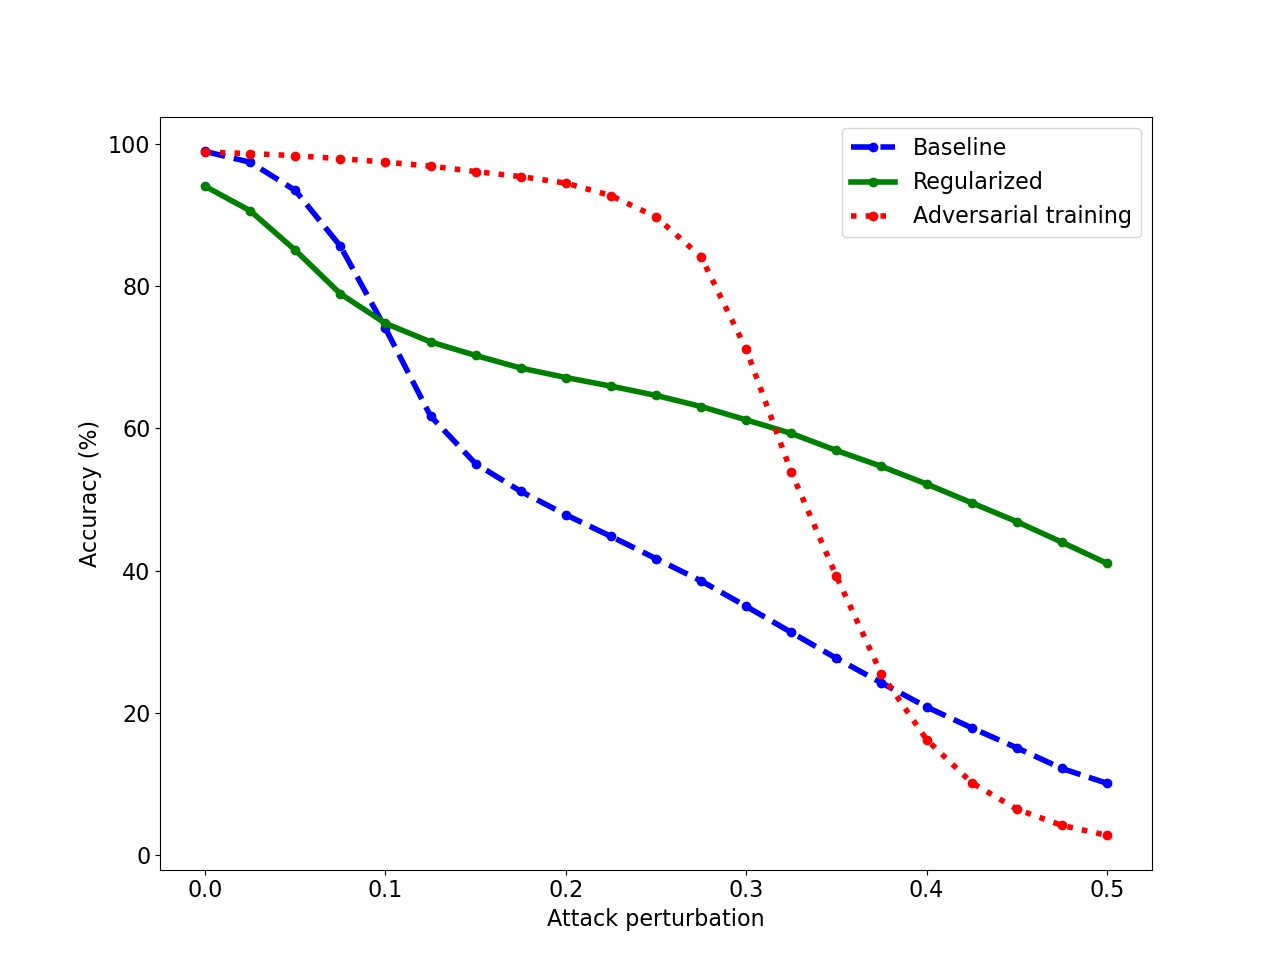
\includegraphics[width=0.55\textwidth]{figures/iso_8_vanilla_2_adv_train_pgd.png}}
%  \vspace{1.5cm}
  \caption{Accuracy of the baseline (dashed, blue), regularized (solid, green), and adversarially trained (dotted, red) models for various attack perturbations on the MNIST dataset. The perturbations are obtained with PGD using $l_\infty$ norm.}
  \label{fig:pgd}
%
\end{figure}



To measure the adversarial robustness of the models, we used the PGD attack with the $l_\infty$ norm, 40 iterations, and a step size of 0.01. The $l_\infty$ norm yields the hardest possible attack for our method, and corresponds more to the human notion of ``indistinguishable images" than the $l_2$ norm. The attacks are performed on the test set, and only on images that were correctly classified by each model. The results are reported in Fig. \ref{fig:pgd}. The regularized model has a slightly lower accuracy than the baseline model for small perturbations, but the baseline model suffers a drop in accuracy above attack level $\epsilon = 0.1$. Adversarial training achieves high accuracy for small to medium-sized perturbations but the accuracy decreases sharply above $\epsilon=0.3$. The regularized model remains robust even for large perturbations. The baseline model reaches 50\% accuracy at $\epsilon=0.2$ and the adversarially trained model at $\epsilon=0.325$, while the regularized model reaches 50\% accuracy at $\epsilon=0.4$.

Table \ref{tab:robust} provides more results against AutoAttack (AA) \citep{croceReliableEvaluationAdversarial2020}, which was designed to offer a more reliable evaluation of adversarial robustness. For fair comparison, and in addition to a baseline model (BASE), we compare the partial isometry defense with several other computationally efficient: distillation (DIST) \citep{papernotDistillationDefenseAdversarial2016}, Jacobian regularization (JAC) \citep{hoffmanRobustLearningJacobian2019}, which also relies on the Jacobian matrix of the network, and Fisher information regularization (FIR) \citep{shenDefendingAdversarialAttacks2019}, which also leverages information geometry. We also consider an adversarially trained (AT) model using PGD. We see that the DIST method, which is the best method outside AT against FGSM (not reported), drops below BASE against AA. This is also the case of FIR. ISO is the best defense not relying on adversarial training. In future work, ISO may be combined with AT to further boost performance.

\begin{table}
\begin{center}\scriptsize
    \begin{tabular}{|l||c|c|c|c|c|c|}\hline
        \bf Defense & \bf BASE & \bf ISO & \bf DIST & \bf JAC & \bf FIR & \bf AT \\
        \hline
        \hline
        Clean & 99.01 & 96.51 & 98.81 & 98.95 & 98.84 & 98.98 \\
        \hline
        AA-$L_2$ (0.15) & 35.70 & 43.38 & 35.35 & 38.74 & 1.68 & 73.34 \\
        \hline
        AA-$L_\infty$ (1.5) & 10.38 & 22.15 & 9.63 & 13.30 & 0.03 & 95.43 \\
        \hline
    \end{tabular}
    \caption{Clean and robust accuracy on MNIST against AA, averaged over 10 runs. The number in parentheses is the attack strength.}
    \label{tab:robust}
\end{center}
\end{table}

\subsection{Experiments on CIFAR-10 dataset}

We consider\footnote{Code available here: \url{https://github.com/lshigarrier/iso_defense.git}} a DenseNet121 model fine-tuned on CIFAR-10 using pre-trained weights for ImageNet. As for the MNIST experiments, we compare the partial isometry defense with distillation (DIST), Jacobian regularization (JAC), and Fisher information regularization (FIR). Here, the adversarial training (AT) relies on FGSM attack \citep{wong2020}. All defenses are compared against PGD for various attack strengths. The results are reported in Table \ref{tab:res}. The defenses are evaluated in a ``gray-box" setting where the adversary can access the architecture and the data but not the weights. More precisely, the adversarial examples are crafted from the test set of CIFAR-10 using another unregularized DenseNet121 model. AT is the more robust method, but ISO achieves a robust accuracy 30\% higher than the next best analogous method (FIR).

One of our goals is to provide alternatives to adversarial training (AT). Besides high computational cost, AT suffers from several limitations: it only robustifies against the chosen attack at the chosen budget, and does not offer robustness guarantees. For example, under Gaussian noise, AT accuracy decreases \emph{faster} than baseline accuracy (i.e., no defense). Achieving high robustness accuracy against specific attacks on specific benchmark is insufficient and misleading to measure the true robustness of the evaluated model. Our method offers a new point of view that can be extended to certified defense methods in future works.

\begin{table}
\begin{center}\scriptsize
    \begin{tabular}{|l||c|c|c|c|c|c|}\hline
        \bf Defense & \bf BASE & \bf ISO & \bf DIST & \bf JAC & \bf FIR & \bf AT \\
        \hline
        \hline
        Clean & 92.93 & 76.86 & 84.96 & 86.17 & 89.98 & 80.78 \\
        \hline
        PGD (4/255) & 2.49 & 40.17 & 7.54 & 8.56 & 9.74 & 68.82 \\
        \hline
        PGD (8/255) & 0.47 & 39.68 & 3.35 & 3.66 & 4.05 & 66.61 \\
        \hline
    \end{tabular}
    \caption{Clean and robust accuracy on CIFAR-10 against PGD. The number in parentheses is the attack strength.}
    \label{tab:res}
\end{center}
\end{table}

\section{Discussion and related work}
\label{sec:dis}

In 2019, Zhao \emph{et al.} \citep{zhaoAdversarialAttackDetection2019} proposed to use the Fisher information metric in the setting of adversarial attacks. They used the eigenvector associated to the largest eigenvalue of the pullback of the FIM as an attack direction. Following their work, Shen \emph{et al.} \citep{shenDefendingAdversarialAttacks2019} suggested a defense mechanism by suppressing the largest eigenvalue of the FIM. They upper-bounded the largest eigenvalue by the trace of the FIM. As in our work, they added a regularization term to encourage the model to have smaller eigenvalues. Moreover, they showed that their approach is equivalent to label smoothing \citep{NEURIPS2019_f1748d6b}. In our framework, their method consists in expanding the geodesic ball $\tilde{b}(x, \delta)$ as much as possible. However, their approach does not guarantee that the constraint imposed on the model will not harm the accuracy more than necessary. In our framework, the matrix $PJ$ (compared with $\delta/\epsilon$) informs the model on the precise restriction that must be imposed to achieve adversarial robustness in the $l_2$ ball of radius $\epsilon$. 

Cisse \emph{et al.} \citep{cisseParsevalNetworksImproving2017} introduced an other adversarial defense called  \emph{Parseval networks}. To achieve adversarial robustness, the authors aim at controlling the Lipschitz constant of each layer of the model to be close to unity. This is achieved by constraining the weight matrix of each layer to be a \emph{Parseval tight frame}, which is synonymous with semi-orthogonal matrix. Since the Jacobian matrix of the entire model with respect to the input is almost the product of the weight matrices, the Parseval network defense is similar to our proposed defense, albeit with completely different rationales. This suggests that geometric reasoning could successfully supplement the line of work on Lipschitz constants of neural networks, such as in \citep{bethunePayAttentionYour2022}.

Following another line of work, Hoffman \emph{et al.} \citep{hoffmanRobustLearningJacobian2019} advanced a Jacobian regularization to improve adversarial robustness. Their regularization consists in using the Frobenius norm of the input-output Jacobian matrix. To avoid computing the true Frobenius norm, they relied on random projections, which are shown to be both efficient and accurate. This method is similar to the method of Shen \emph{et al.} \citep{shenDefendingAdversarialAttacks2019} in the sense that it will also increase the radius of the geodesic ball. However, the Jacobian regularization does not take into account the geometry of the output space (i.e., the Fisher information metric) and assumes that the probability simplex $\Delta^m$ is Euclidean.

Although this study focuses on $l_2$ norm robustness, it must be pointed out that there are other ``distinguishability" measures that can be used to study adversarial robustness, including all other $l_p$ norms. In particular, the $l_\infty$ norm is often considered to be the most natural choice when working with images. However, the $l_\infty$ norm is not induced by any inner product, and hence, there is no Riemannian metric that induces the $l_\infty$ norm. However, given an $l_\infty$ budget $\epsilon_\infty$, we can choose an $l_2$ budget $\epsilon_2 = \sqrt{n} \epsilon_\infty$ such that any attack in the $\epsilon_\infty$ budget will also respect the $\epsilon_2$ budget. When working on images, other dissimilarity measures are: rotations, deformations, or color changes of the original image. Contrary to the $l_2$ or $l_\infty$, these measures are not based on a pixel-based coordinate system. However, it is possible to define \emph{unrestricted attacks} based on these spatial dissimilarities, for example in \citep{xiao2018spatially}. 

In this work, we derived the partial isometry regularization for a classification task. The method can be extended to regression tasks by considering the family of multivariate normal distributions as the output space. On the probability simplex $\Delta^m$, the FIM is a metric with constant positive curvature, while it has constant negative curvature on the manifold of multivariate normal distributions \citep{skovgaardRiemannianGeometryMultivariate1984}.

Finally, the precise quantification of the robustness condition presented in Eq. (\ref{eq:robust_condition}) and Proposition \ref{th:main} paves the way to the development of a certified defense \citep{cohenCertifiedAdversarialRobustness2019} in this framework. By strongly enforcing Proposition \ref{th:main} on a chosen proportion of the training set, it may be possible to maximize the accuracy under the constraint of a chosen robustness level, which offers another solution to the robustness-accuracy trade-off \citep{pmlr-v97-zhang19p}, \citep{tsipras2018robustness}. Certifiable defenses are a require step for the deployment of deep learning models in critical domains and missions, such as civil aviation, security, defense and healthcare, where a certification may be required to ensure a sufficient level of trustworthiness.

\section{Conclusion and future work}
\label{seq:conclu}

In this paper, we introduced an information geometric approach to the problem of adversarial robustness in machine learning models. The proposed defense consists of enforcing a partial isometry between the input space endowed with the Euclidean metric and the probability simplex endowed with the Fisher information metric. We subsequently derived a regularization term to achieve robustness during training. The proposed strategy is tested on the MNIST and CIFAR-10 datasets, and shows considerable increase in robustness without harming the accuracy. Future works will evaluate the method on other benchmarks and real-world datasets. Several attack methods will also be considered in addition to PGD and AutoAttack. Although this work focuses on $l_2$ norm robustness, future work would consider other ``distinguishability" measures. 

Our work extends a recent, promising but under-studied framework for adversarial robustness based on information geometric tools. The FIM has already been harnessed to develop attacks \citep{zhaoAdversarialAttackDetection2019} and defenses \citep{picotAdversarialRobustnessFisherRao2022, shenDefendingAdversarialAttacks2019} but a precise robustness analysis is yet to be proposed. Our work is a step towards the development of such analysis which may yield certified guarantees relying on these geometric tools. The study of adversarial robustness, which is non-local by definition and contrary to accuracy, should benefit greatly from a geometrical vision. However, the current literature on adversarial robustness is mainly concerned with the FIM and its spectrum (which are very local objects) without unfolding the full arsenal developed in information geometry. In our work, we demonstrate the usefulness of such approach by developing a preliminary robustification method. Model robustification is a hard, unsolved yet vital problem to ensure the trustworthiness of deep learning tools in safety-critical applications. Our framework could be extended and applied to existing certification strategies, such as Lipschitz-based \citep{leinoGloballyRobustNeuralNetworks2021} or randomized smoothing \citep{cohenCertifiedAdversarialRobustness2019} where statistical models naturally appear.

% --------------------------------------------------------------------------------------------------------------

\section{Proofs}
\label{sec:proof}

\begin{proof}[Proof of Proposition \ref{prop:as1}]
    (\ref{eq:as1-2}) $\Rightarrow$ (\ref{eq:as1}]). Assume (\ref{eq:as1-2}). Let $v \in \overline{\B}_x(0, \epsilon)$. Thus $\gb_x(v,v) \leq \epsilon^2$. We have:
    \begin{equation*}
        \tilde{g}_x(v,v) \leq \frac{\delta^2}{\epsilon^2} \gb_x(v,v) \leq \frac{\delta^2}{\epsilon^2} \epsilon^2 = \delta^2.
    \end{equation*}
    Thus $v \in \widetilde{\B}_x(0, \delta)$. \\
    (\ref{eq:as1}) $\Rightarrow$ (\ref{eq:as1-2}]). Assume (\ref{eq:as1}). Let $v \in T_x\X$. Define $w = \epsilon \, v / \sqrt{\gb_x(v,v)}$. Then $\gb_x(w,w) = \epsilon^2$. Thus, $w \in \overline{\B}_x(0, \epsilon)$. Hence, $w \in \widetilde{\B}_x(0, \delta)$. Thus, $\tilde{g}_x(w,w) < \delta^2$. Finally, we have:
    \begin{equation*}
        \tilde{g}_x(w,w) = \frac{\epsilon^2}{\gb_x(v,v)} \tilde{g}_x(v,v) < \delta^2.
    \end{equation*}
    We obtain Equation (\ref{eq:as1-2}) by multiplying by $\gb_x(v,v)/\epsilon^2$.
\end{proof}

\begin{proof}[Proof of Proposition \ref{prop:embed}]
    We need to show that $\mu^* \gb = g$. Using the coordinates $\theta$ on $\Delta^m$ (Definition \ref{def:simplex}) and the standard coordinates on $\R^c$, and writing $f(x) = \theta_0 = (\theta^1_0, \dots, \theta^m_0)$ we have:
    \begin{align*}
        G_{ij} &= G_{\theta_0, ij}, \\
        &= \sum_{\alpha=1}^c \sum_{\beta=1}^c \frac{\partial \mu^\alpha(\theta_0)}{\partial \theta^i} \frac{\partial \mu^\beta(\theta_0)}{\partial \theta^j} \delta_{\alpha \beta}, \\
        &= \sum_{\alpha=1}^c \frac{\partial \mu^\alpha(\theta_0)}{\partial \theta^i} \frac{\partial \mu^\alpha(\theta_0)}{\partial \theta^j}.
    \end{align*}
    For $i=1, \dots, m$ and $\alpha=1, \dots, m$ we have:
    \begin{equation*}
        \frac{\partial \mu^\alpha(\theta_0)}{\partial \theta^i} = \frac{\delta_{i \alpha}}{\sqrt{\theta^i_0}},
    \end{equation*}
    and for $\alpha = c$:
    \begin{equation*}
        \frac{\partial \mu^c(\theta_0)}{\partial \theta^i} = -\frac{1}{\sqrt{\theta^c_0}},
    \end{equation*}
    with $\theta^c_0 = \sqrt{1 - \sum_{i=1}^m \theta^i_0}$. Thus:
    \begin{equation*}
        G_{\theta, ij} = \frac{\delta_{ij}}{\theta^i_0} + \frac{1}{\theta^c_0},
    \end{equation*}
    which is the FIM as defined in Definition \ref{def:fim}.
\end{proof}

\begin{proof}[Proof of Proposition \ref{prop:stereo}]
    For $i=1, \dots, m$, the inverse transformation of $\tau(\mu)$ is:
    \begin{equation}
        \label{eq:inverse_change}
        \mu^i(\tau) = \frac{2\tau^i}{1+\left\|\tau/2\right\|^2},
    \end{equation}
    and:
    \begin{equation}
        \label{eq:inverse_change_2}
        \mu^c(\tau) = 2 \frac{\left\|\tau/2\right\|^2-1}{\left\|\tau/2\right\|^2+1}.
    \end{equation}
    The proofs of Eqs. (\ref{eq:inverse_change}) and (\ref{eq:inverse_change_2}) are provided below. \\
    Moreover, according to Proposition \ref{prop:embed}, the FIM in the coordinates $(\mu^1, \dots, \mu^m)$ is the metric induced on $\mu(\Delta^m)$ by the identity matrix (i.e., the Euclidean metric) of $\R^c$. Hence, we have:
    \begin{align*}
        G_{\tau, ij} &= \sum_{\alpha=1}^c \sum_{\beta=1}^c \frac{\partial \mu^\alpha(\tau)}{\partial \tau^i} \frac{\partial \mu^\beta(\tau)}{\partial \tau^j} \delta_{\alpha \beta}, \\
        &= \sum_{\alpha=1}^c \frac{\partial \mu^\alpha(\tau)}{\partial \tau^i} \frac{\partial \mu^\alpha(\tau)}{\partial \tau^j}.
    \end{align*}
    For $i=1, \dots, m$ and $\alpha=1, \dots, m$ we have:
    \begin{equation*}
        \frac{\partial \mu^\alpha(\tau)}{\partial \tau^i} = \frac{2}{1+\|\tau/2\|^2}\left(\delta_{i \alpha} - \frac{\tau^\alpha \tau^i}{2\left(1+\|\tau/2\|^2\right)} \right),
    \end{equation*}
    and for $\alpha = c$:
    \begin{equation*}
        \frac{\partial \mu^c(\tau)}{\partial \tau^i} = \frac{2\tau^i}{\left(1+\|\tau/2\|^2\right)^2},
    \end{equation*}
    Thus:
    \footnotesize
    \begin{align*}
        G_{\tau, ij} =& \frac{4}{\left(1+\|\tau/2\|^2\right)^2} \Biggl( \sum_{\alpha=1}^m \Biggl\{ \delta_{i \alpha} \delta_{j \alpha} - \frac{\delta_{i \alpha} \tau^j \tau^\alpha}{2\left(1+\|\tau/2\|^2\right)} \\
        &- \frac{\delta_{j \alpha} \tau^i \tau^\alpha}{2\left(1+\|\tau/2\|^2\right)} + \frac{\tau^i \tau^j \left(\tau^\alpha\right)^2}{4\left(1 + \|\tau/2\|^2\right)^2}\Biggl\} + \frac{\tau^i \tau^j}{\left(1 + \|\tau/2\|^2\right)^2} \Biggl), \\
        =& \frac{4}{\left(1+\|\tau/2\|^2\right)^2}\Biggl( \delta_{ij} - \frac{\tau^i \tau^j}{1+\|\tau/2\|^2} + \frac{\tau^i \tau^j \|\tau/2\|^2}{\left(1 + \|\tau/2\|^2\right)^2} \\
        &+ \frac{\tau^i \tau^j}{\left(1 + \|\tau/2\|^2\right)^2}\Biggl), \\
        =& \frac{4}{\left(1+\|\tau/2\|^2\right)^2}\left( \delta_{ij} - \frac{\tau^i \tau^j}{1+\|\tau/2\|^2} + \frac{\tau^i \tau^j}{1 + \|\tau/2\|^2}\right), \\
        =& \frac{4}{\left(1+\|\tau/2\|^2\right)^2} \delta_{ij}.
    \end{align*}
    \normalsize
\end{proof}

\begin{proof}[Proof of Eqs. (\ref{eq:inverse_change}) and (\ref{eq:inverse_change_2})]
    We have $\tau^i(\mu) = \lambda \mu^i$ with $\lambda = 2/\left(2-\mu^c\right)$. Let us express $\mu^c$ as a function of $\tau$. We have:
    \begin{equation*}
        \|\tau\|^2 = \sum_{i=1}^m (\tau^i)^2 = \lambda^2 \|\mu\|^2.
    \end{equation*}
    Since $\mu$ belongs to the sphere of radius 2, we have $\|\mu\|^2+(\mu^c)^2=4$. Thus:
    \begin{equation*}
         \|\tau\|^2 = \lambda^2 \left(4 - (\mu^c)^2\right) = 4\frac{4 - (\mu^c)^2}{\left(2 - \mu^c\right)^2} = 4 \frac{2 + \mu^c}{2 - \mu^c}.
    \end{equation*}
    Isolating $\mu^c$, we get:
    \begin{equation}
        \label{eq:tau-1_1}
        \mu^c(\tau) = \frac{2\|\tau\|^2-8}{\|\tau\|^2+4} = 2 \frac{\left\|\tau/2\right\|^2-1}{\left\|\tau/2\right\|^2+1}.
    \end{equation}
    Now, we can replace $\mu^c$ into the expression of $\lambda$. We obtain $\lambda = \left(1+\|\tau/2\|^2\right)/2$, and thus:
    \begin{equation}
        \label{eq:tau-1_2}
        \mu^i(\tau) = \frac{\tau^i}{\lambda} = \frac{2\tau^i}{1+\|\tau/2\|^2}
    \end{equation}
\end{proof}

\begin{proof}[Proof of Proposition \ref{prop:matrix_p}]
    We have:
    \begin{equation*}
        \tau^i(\theta) = 2\sqrt{\theta^i}/\left(1-\sqrt{\theta^c}\right).    
    \end{equation*}
    Thus:
    \begin{align*}
        \left\|\frac{\tau(\theta)}{2}\right\|^2 &= \sum_{i=1}^m \frac{\tau^i(\theta)^2}{4}, \\
        &= \frac{\sum_{i=1}^m \theta^i}{\left(1- \sqrt{\theta^c}\right)^2}, \\
        &= \frac{1 - \theta^c}{\left(1- \sqrt{\theta^c}\right)^2}, \\
        &= \frac{1+\sqrt{\theta^c}}{1-\sqrt{\theta^c}}.  
    \end{align*}
    Hence, for any $i = 1, \dots, m$:
    \begin{equation}
    \label{eq:kappa}
        \frac{2}{1+\|\tau(\theta)/2\|^2} = 1 - \sqrt{\theta^c} = \frac{2\sqrt{\theta^i}}{\tau^i(\theta)}.
    \end{equation}
    Now, we compute $\widetilde{J}$. Let $i$ and $j$ in $\{1, \dots, m\}$:
    \begin{align}
        \frac{\partial \tau^i(\theta)}{\partial \theta^j} &= \frac{\delta_{ij}}{\sqrt{\theta^i}\left(1-\sqrt{\theta^c}\right)} - \frac{\sqrt{\theta^i}}{\sqrt{\theta^c}\left(1-\sqrt{\theta^c}\right)^2}, \\
        \label{eq:jac_tau}
        &= \frac{\tau^i(\theta)}{2}\left(\frac{\delta_{ij}}{\theta^i} - \frac{\tau^i(\theta)}{2\sqrt{\theta^i \theta^c}}\right).
    \end{align}
    Replacing Eqs. (\ref{eq:kappa}) and (\ref{eq:jac_tau}) into Eq. (\ref{eq:matrix_p}) yields the result.
\end{proof}

\begin{proof}[Proof of Fact \ref{fact1}]
    We prove the third equality (the second equality is a well-known fact of linear algebra). \\
    Let $u \in \ker J$. Then $J^T G J u = 0$, thus $u \in \ker(J^T G J)$. Hence $\left(\ker(J^T G J)\right)^\perp \subseteq \left(\ker(J)\right)^\perp$. \\
    Let $v \in \ker J^T G J$. Since $G$ is symmetric positive-definite, the function $w \mapsto N(w) = \sqrt{w^TGw}$ is a norm. We have $0 = v^T J^T G J v= N(J v)^2$. The positive-definiteness of the norm $N$ implies $J v = 0$. Thus, $v \in \ker J$. Hence $\left(\ker(J)\right)^\perp \subseteq \left(\ker(J^T G J)\right)^\perp  $.
\end{proof}

\begin{proof}[Proof of Proposition \ref{prop:as2}]
The implication (\ref{eq:as2-2}) $\Rightarrow$ (\ref{eq:as2}]) is immediate (by double inclusion). \\
Now, assume (\ref{eq:as2}]) holds. Let $v \in D$. Define $w_1 = \epsilon \, v/\sqrt{\gb_x(v,v)}$ and $w_2 = \epsilon \, v  /\sqrt{\tilde{g}_x(v,v)}$. Then, with a similar argument as in the proof of Proposition \ref{prop:as1}, we can obtain Eq. (\ref{eq:as2-2}). Note that $w_2$ is well defined because $v \notin \ker(J)$.
\end{proof}

\begin{proof}[Proof of Proposition \ref{th:main}]
    \textbf{Let us first introduce the polar decomposition}. \\
    Let $A$ be a $m \times d$ matrix. \\
    Define the absolute value\footnote{The square root of $A^TA$ is well defined because it is a positive semidefinite matrix.} of $A$ by $|A| = (A^TA)^{\frac{1}{2}}$. \\
    Define the linear map $u : \rg(|A|) \rightarrow \rg(A)$ by $u(|A|x) = Ax$ for any $x \in \R^d$. \\
    Using the fact that $|A|$ is symmetric, we have that $\|Ax\|^2 = x^T A^T A x = (A^TAx)^T x = (|A|^2x)^Tx = x^T |A|^T |A| x = \||A|x\|^2$, thus $u$ is an isometry\footnote{We can arbitrarily extend $u$ on the entire $\R^d$, e.g., by setting $\ker(u) = \ker(|A|)$.}. \\
    Let $U$ be the matrix associated to $u$ in the canonical basis. \\
    \textbf{We now prove the main result}. \\
    Let $A=PJ$. Using the polar decomposition, we have
    \begin{equation*}
        PJ = U |PJ|,    
    \end{equation*}
    where $U$ is an isometry from $\rg(|PJ|) = (\ker|PJ|)^\perp = (\ker(PJ))^\perp = (\ker(J))^\perp = D$ to $\rg(PJ) = \R^m$ (using our assumption that $\rk(J) = m$). Transposing this relation, we obtain:
    \begin{equation*}
        J^TP^T=|PJ|U^T.    
    \end{equation*}
    Hence, by multiplying both relations, we have:
    \begin{equation}
        \label{eq:uniteq}
        PJJ^TP^T = U |PJ|^2 U^T = U J^TP^TPJ U^T
    \end{equation}
    Assume that $(ii)$ holds, i.e., $PJJ^TP = I_m$. Then:
    \begin{equation*}
        J^T G J = J^TP^TPJ = U^T PJJ^TP^T U = U^T U.
    \end{equation*}
    Since $U$ is an isometry from $D$ to $\R^m$, then $U^TU$ is the projection onto $D$, denoted $\Pi_D$. Thus, we have $J^TGJ = \Pi_D$ which is $(i)$. \\
    Now, assume that $(i)$ holds, i.e., $J^TP^TPJ = \Pi_D$ where $\Pi_D$ is the projection onto $D$. We have:
    \begin{equation*}
        PJJ^TP^T = UJ^TP^TPJU^T =U\Pi_DU^T. 
    \end{equation*}
    Since $\rg(U^T) = D$, then $\Pi_D U^T = U^T$. Since $U$ is an isometry from $D$ to $\R^m$, then $UU^T=I_m$. Thus, $PJJ^TP^T = I_m$ which is $(ii)$.
\end{proof}



%%%%%%%%%%%%%%%%%%%%%%%%%%%%%%%%%%%%%%%%%%
\authorcontributions{The authors contribute equally in this work.}

\funding{``This research received no external funding'' }

%\institutionalreview{In this section, you should add the Institutional Review Board Statement and approval number, if relevant to your study. You might choose to exclude this statement if the study did not require ethical approval. Please note that the Editorial Office might ask you for further information. Please add “The study was conducted in accordance with the Declaration of Helsinki, and approved by the Institutional Review Board (or Ethics Committee) of NAME OF INSTITUTE (protocol code XXX and date of approval).” for studies involving humans. OR “The animal study protocol was approved by the Institutional Review Board (or Ethics Committee) of NAME OF INSTITUTE (protocol code XXX and date of approval).” for studies involving animals. OR “Ethical review and approval were waived for this study due to REASON (please provide a detailed justification).” OR “Not applicable” for studies not involving humans or animals.}

%\informedconsent{Any research article describing a study involving humans should contain this statement. Please add ``Informed consent was obtained from all subjects involved in the study.'' OR ``Patient consent was waived due to REASON (please provide a detailed justification).'' OR ``Not applicable'' for studies not involving humans. You might also choose to exclude this statement if the study did not involve humans.

%Written informed consent for publication must be obtained from participating patients who can be identified (including by the patients themselves). Please state ``Written informed consent has been obtained from the patient(s) to publish this paper'' if applicable.}

%\dataavailability{We encourage all authors of articles published in MDPI journals to share their research data. In this section, please provide details regarding where data supporting reported results can be found, including links to publicly archived datasets analyzed or generated during the study. Where no new data were created, or where data is unavailable due to privacy or ethical restrictions, a statement is still required. Suggested Data Availability Statements are available in section ``MDPI Research Data Policies'' at \url{https://www.mdpi.com/ethics}.} 

% Only for journal Nursing Reports
%\publicinvolvement{Please describe how the public (patients, consumers, carers) were involved in the research. Consider reporting against the GRIPP2 (Guidance for Reporting Involvement of Patients and the Public) checklist. If the public were not involved in any aspect of the research add: ``No public involvement in any aspect of this research''.}

% Only for journal Nursing Reports
%\guidelinesstandards{Please add a statement indicating which reporting guideline was used when drafting the report. For example, ``This manuscript was drafted against the XXX (the full name of reporting guidelines and citation) for XXX (type of research) research''. A complete list of reporting guidelines can be accessed via the equator network: \url{https://www.equator-network.org/}.}

%\acknowledgments{In this section you can acknowledge any support given which is not covered by the author contribution or funding sections. This may include administrative and technical support, or donations in kind (e.g., materials used for experiments).}

\conflictsofinterest{``The authors declare no conflict of interest.''}

%%%%%%%%%%%%%%%%%%%%%%%%%%%%%%%%%%%%%%%%%%
%% Optional
%\sampleavailability{Samples of the compounds ... are available from the authors.}

%% Only for journal Encyclopedia
%\entrylink{The Link to this entry published on the encyclopedia platform.}

% \abbreviations{Abbreviations}{
% The following abbreviations are used in this manuscript:\\

% \noindent 
% \begin{tabular}{@{}ll}
% MDPI & Multidisciplinary Digital Publishing Institute\\
% DOAJ & Directory of open access journals\\
% TLA & Three letter acronym\\
% LD & Linear dichroism
% \end{tabular}
% }

%%%%%%%%%%%%%%%%%%%%%%%%%%%%%%%%%%%%%%%%%%
%% Optional
% \appendixtitles{no} % Leave argument "no" if all appendix headings stay EMPTY (then no dot is printed after "Appendix A"). If the appendix sections contain a heading then change the argument to "yes".
% \appendixstart
% \appendix
% \section[\appendixname~\thesection]{}
% \subsection[\appendixname~\thesubsection]{}
% The appendix is an optional section that can contain details and data supplemental to the main text---for example, explanations of experimental details that would disrupt the flow of the main text but nonetheless remain crucial to understanding and reproducing the research shown; figures of replicates for experiments of which representative data are shown in the main text can be added here if brief, or as Supplementary Data. Mathematical proofs of results not central to the paper can be added as an appendix.

% \begin{table}[H] 
% \caption{This is a table caption.\label{tab5}}
% \newcolumntype{C}{>{\centering\arraybackslash}X}
% \begin{tabularx}{\textwidth}{CCC}
% \toprule
% \textbf{Title 1}	& \textbf{Title 2}	& \textbf{Title 3}\\
% \midrule
% Entry 1		& Data			& Data\\
% Entry 2		& Data			& Data\\
% \bottomrule
% \end{tabularx}
% \end{table}

% \section[\appendixname~\thesection]{}
% All appendix sections must be cited in the main text. In the appendices, Figures, Tables, etc. should be labeled, starting with ``A''---e.g., Figure A1, Figure A2, etc.

%%%%%%%%%%%%%%%%%%%%%%%%%%%%%%%%%%%%%%%%%%
\begin{adjustwidth}{-\extralength}{0cm}
%\printendnotes[custom] % Un-comment to print a list of endnotes

\reftitle{References}

% Please provide either the correct journal abbreviation (e.g. according to the “List of Title Word Abbreviations” http://www.issn.org/services/online-services/access-to-the-ltwa/) or the full name of the journal.
% Citations and References in Supplementary files are permitted provided that they also appear in the reference list here. 

%=====================================
% References, variant A: external bibliography
%=====================================
\bibliography{references.bib}

%=====================================
% References, variant B: internal bibliography
%=====================================
% \begin{thebibliography}{999}
% % Reference 1
% \bibitem[Author1(year)]{ref-journal}
% Author~1, T. The title of the cited article. {\em Journal Abbreviation} {\bf 2008}, {\em 10}, 142--149.
% % Reference 2
% \bibitem[Author2(year)]{ref-book1}
% Author~2, L. The title of the cited contribution. In {\em The Book Title}; Editor 1, F., Editor 2, A., Eds.; Publishing House: City, Country, 2007; pp. 32--58.
% % Reference 3
% \bibitem[Author3(year)]{ref-book2}
% Author 1, A.; Author 2, B. \textit{Book Title}, 3rd ed.; Publisher: Publisher Location, Country, 2008; pp. 154--196.
% % Reference 4
% \bibitem[Author4(year)]{ref-unpublish}
% Author 1, A.B.; Author 2, C. Title of Unpublished Work. \textit{Abbreviated Journal Name} year, \textit{phrase indicating stage of publication (submitted; accepted; in press)}.
% % Reference 5
% \bibitem[Author5(year)]{ref-communication}
% Author 1, A.B. (University, City, State, Country); Author 2, C. (Institute, City, State, Country). Personal communication, 2012.
% % Reference 6
% \bibitem[Author6(year)]{ref-proceeding}
% Author 1, A.B.; Author 2, C.D.; Author 3, E.F. Title of presentation. In Proceedings of the Name of the Conference, Location of Conference, Country, Date of Conference (Day Month Year); Abstract Number (optional), Pagination (optional).
% % Reference 7
% \bibitem[Author7(year)]{ref-thesis}
% Author 1, A.B. Title of Thesis. Level of Thesis, Degree-Granting University, Location of University, Date of Completion.
% % Reference 8
% \bibitem[Author8(year)]{ref-url}
% Title of Site. Available online: URL (accessed on Day Month Year).
% \end{thebibliography}

% If authors have biography, please use the format below
%\section*{Short Biography of Authors}
%\bio
%{\raisebox{-0.35cm}{\includegraphics[width=3.5cm,height=5.3cm,clip,keepaspectratio]{Definitions/author1.pdf}}}
%{\textbf{Firstname Lastname} Biography of first author}
%
%\bio
%{\raisebox{-0.35cm}{\includegraphics[width=3.5cm,height=5.3cm,clip,keepaspectratio]{Definitions/author2.jpg}}}
%{\textbf{Firstname Lastname} Biography of second author}

% For the MDPI journals use author-date citation, please follow the formatting guidelines on http://www.mdpi.com/authors/references
% To cite two works by the same author: \citeauthor{ref-journal-1a} (\citeyear{ref-journal-1a}, \citeyear{ref-journal-1b}). This produces: Whittaker (1967, 1975)
% To cite two works by the same author with specific pages: \citeauthor{ref-journal-3a} (\citeyear{ref-journal-3a}, p. 328; \citeyear{ref-journal-3b}, p.475). This produces: Wong (1999, p. 328; 2000, p. 475)

%%%%%%%%%%%%%%%%%%%%%%%%%%%%%%%%%%%%%%%%%%
%% for journal Sci
%\reviewreports{\\
%Reviewer 1 comments and authors’ response\\
%Reviewer 2 comments and authors’ response\\
%Reviewer 3 comments and authors’ response
%}
%%%%%%%%%%%%%%%%%%%%%%%%%%%%%%%%%%%%%%%%%%
\PublishersNote{}
\end{adjustwidth}
\end{document}
